%!TEX root = ../thesis.tex

\section{オンライン手法の概要}
従来から提案してきたオンライン手法に関して述べる. オンライン手法では, 地図を用いたルールベース制御器の出力を模倣して, 経路追従行動を獲得する. \figref{Fig:learning}にシステム概要を示す. 学習時は, LiDARとオドメトリを入力として, ROSのnavigation[7]により,目標角速度を求めて,ロボットを経路追従させる. 同時に64×48にリサイズした 3つのカメラ画像(RGB画像)を入力, 目標角速度を出力とするデータを, データセットに加える. そのデータをランダムにピックアップしてリアルタイムに学習する. 左右のカメラ画像に対する目標角速度には, それぞれ経路に戻るためのオフセットを加える. これらは経路から外れた場合に, 経路に戻る行動が選択されるように加えている. \par 一定ステップ数の学習を行った後, 学習したモデルで経路追従できるか確認する. \figref{Fig:test}にシステム概要を示す. 中央のカメラ画像を深層学習器に入力して, 出力された目標角速度を用いてロボットを制御する. なお, 目標の並進速度は0.2[m/s]で一定とする.

\newpage
\begin{figure}[h]
  \centering
  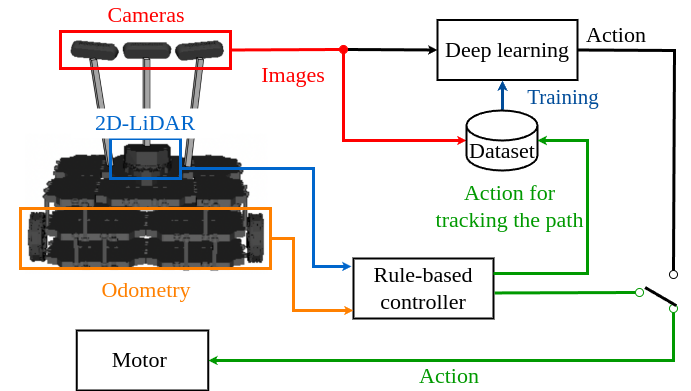
\includegraphics[keepaspectratio, scale=0.45]{images/si2021-okada.png}
  \caption{System configuration during network training}
  \label{Fig:learning}
  \end{figure}

\begin{figure}[h]
  \centering
  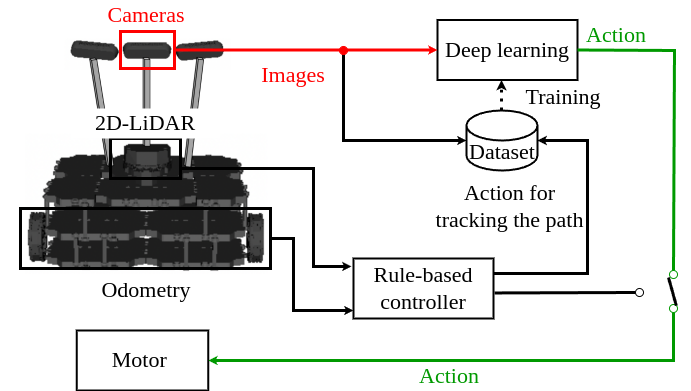
\includegraphics[keepaspectratio, scale=0.45]{images/si2021-okada-test.png}
  % \caption*{(b)Test phase}
  \caption{System configuration after network training}
  \label{Fig:test}
  \end{figure}

  \newpage
\section{ネットワークの構造}
\figref{Fig:cnn}に従来手法で用いたネットワークの構造を示す. 構造は, 入力層1, 畳み込み層3, 全結合層2, 出力層1の計7層から構成されている. また, オンラインで学習が行えるように, ネットワークは畳み込みニューラルネットワーク(CNN)を基にしている. 

\vspace{10mm}
\begin{figure}[h]
  \centering
  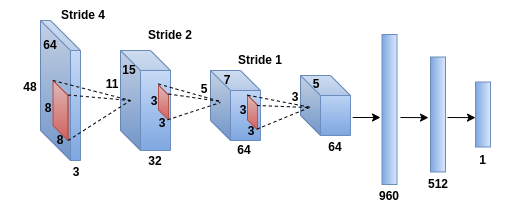
\includegraphics[keepaspectratio, scale=0.6]{images/cnn.png}
  \caption{Structure of network}
  \label{Fig:cnn}
  \end{figure}


